%%%%%%%%%%%%%%%%%%%%%%%%%%%%%%%%%%%%%%%%%
% Beamer Presentation
% LaTeX Template
% Version 1.0 (10/11/12)
%
% This template has been downloaded from:
% http://www.LaTeXTemplates.com
%
% License:
% CC BY-NC-SA 3.0 (http://creativecommons.org/licenses/by-nc-sa/3.0/)
%
%%%%%%%%%%%%%%%%%%%%%%%%%%%%%%%%%%%%%%%%%

%----------------------------------------------------------------------------------------
%	PACKAGES AND THEMES
%----------------------------------------------------------------------------------------

\documentclass{beamer}

\definecolor{dark green}{rgb}{0.0, 0.5, 0.0}

\mode<presentation> {

% The Beamer class comes with a number of default slide themes
% which change the colors and layouts of slides. Below this is a list
% of all the themes, uncomment each in turn to see what they look like.

%\usetheme{default}
%\usetheme{AnnArbor}
%\usetheme{Antibes}
%\usetheme{Bergen}
%\usetheme{Berkeley}
%\usetheme{Berlin}
\usetheme{Boadilla}
%\usetheme{CambridgeUS}
%\usetheme{Copenhagen}
%\usetheme{Darmstadt}
%\usetheme{Dresden}
%\usetheme{Frankfurt}
%\usetheme{Goettingen}
%\usetheme{Hannover}
%\usetheme{Ilmenau}
%\usetheme{JuanLesPins}
%\usetheme{Luebeck}
%\usetheme{Madrid}
%\usetheme{Malmoe}
%\usetheme{Marburg}
%\usetheme{Montpellier}
%\usetheme{PaloAlto}
%\usetheme{Pittsburgh}
%\usetheme{Rochester}
%\usetheme{Singapore}
%\usetheme{Szeged}
%\usetheme{Warsaw}

% As well as themes, the Beamer class has a number of color themes
% for any slide theme. Uncomment each of these in turn to see how it
% changes the colors of your current slide theme.

%\usecolortheme{albatross}
%\usecolortheme{beaver}
%\usecolortheme{beetle}
%\usecolortheme{crane}
%\usecolortheme{dolphin}
%\usecolortheme{dove}
%\usecolortheme{fly}
%\usecolortheme{lily}
%\usecolortheme{orchid}
%\usecolortheme{rose}
%\usecolortheme{seagull}
\usecolortheme{seahorse}
%\usecolortheme{whale}
%\usecolortheme{wolverine}

%\setbeamertemplate{footline} % To remove the footer line in all slides uncomment this line
%\setbeamertemplate{footline}[page number] % To replace the footer line in all slides with a simple slide count uncomment this line

%\setbeamertemplate{navigation symbols}{} % To remove the navigation symbols from the bottom of all slides uncomment this line
}

\usepackage{graphicx} % Allows including images
\usepackage{booktabs} % Allows the use of \toprule, \midrule and \bottomrule in tables
\usepackage{tikz}
\usetikzlibrary{positioning}

%----------------------------------------------------------------------------------------
%	TITLE PAGE
%----------------------------------------------------------------------------------------

\title[Montreal Boroughs]{Where am I? \\Predicting Montreal Boroughs \\from Google Street View Images} % The short title appears at the bottom of every slide, the full title is only on the title page

\author[S. Laflamme, B. Leonard-Cannon, S. Ruan]
{%
   \texorpdfstring{
        \begin{columns}
            \column{.33\linewidth}
            \centering
            {\small Stephanie Laflamme}
            \column{.33\linewidth}
            \centering
            {\small Benedicte Leonard-Cannon}
            \column{.33\linewidth}
            \centering
            {\small Sherry Ruan}
        \end{columns}
   }
   {John Doe \& Jane Doe}
}
\institute[] % Your institution as it will appear on the bottom of every slide, may be shorthand to save space
{
McGill University \\ % Your institution for the title page
COMP 598
}
\date{November 27, 2014} % Date, can be changed to a custom date

\begin{document}

\begin{frame}
\titlepage % Print the title page as the first slide
\end{frame}

%----------------------------------------------------------------------------------------
%	PRESENTATION SLIDES
%----------------------------------------------------------------------------------------

\begin{frame}
\frametitle{Nine Montreal Boroughs}
% images (labeled by neighbourhood)
\centering
\begin{tikzpicture}[on grid,]
\node (downtown) at (0,0) {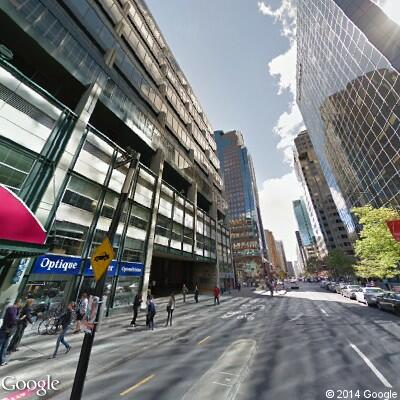
\includegraphics[width=0.21\linewidth]{downtown1.png}}; 
\node (chinatown) [right =2.7 of downtown] {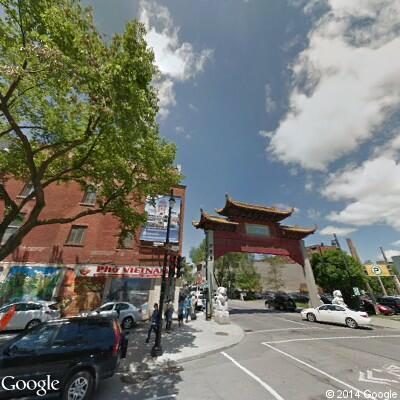
\includegraphics[width=0.21\linewidth]{chinatown.png}}; 
\node (oldmontreal) [right =2.7 of chinatown] {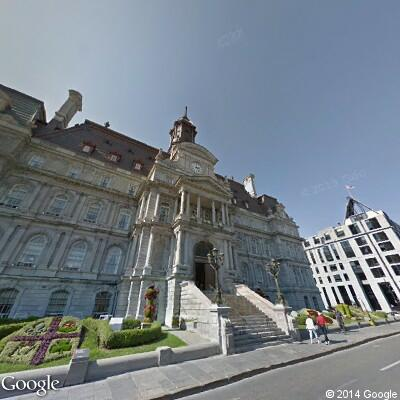
\includegraphics[width=0.21\linewidth]{oldmontreal.png}};
\node (gayvillage) [below =2.7 of downtown] {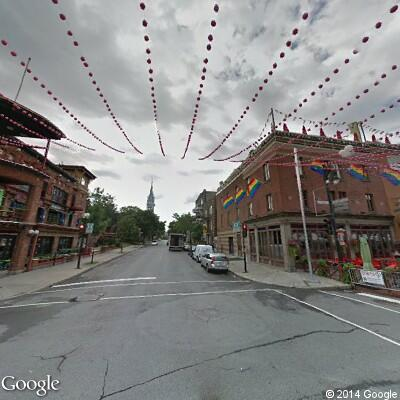
\includegraphics[width=0.21\linewidth]{gayvillage2.png}};
\node (outremont) [right =2.7 of gayvillage] {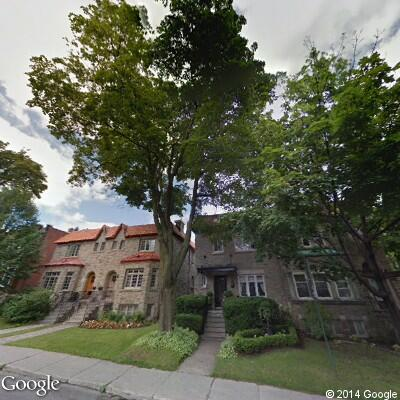
\includegraphics[width=0.21\linewidth]{outremont2.png}};
\node (plateau) [right =2.7 of outremont] {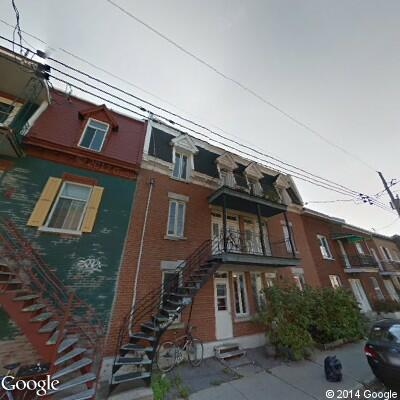
\includegraphics[width=0.21\linewidth]{plateau.png}}; 
\node (westmount) [below =2.7 of gayvillage] {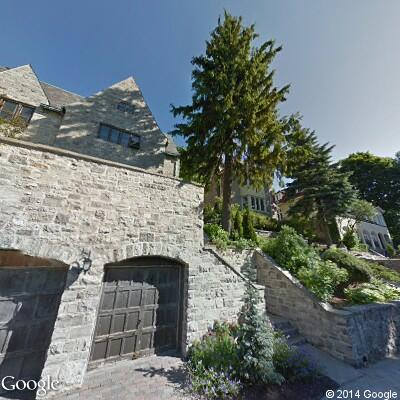
\includegraphics[width=0.21\linewidth]{westmount.png}};
\node (hochelaga) [right =2.7 of westmount] {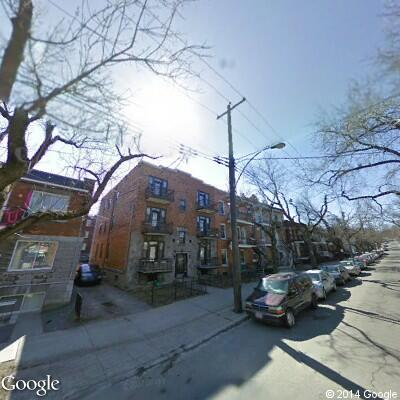
\includegraphics[width=0.21\linewidth]{hochelaga.png}};
\node (montrealnord) [right =2.7 of hochelaga] {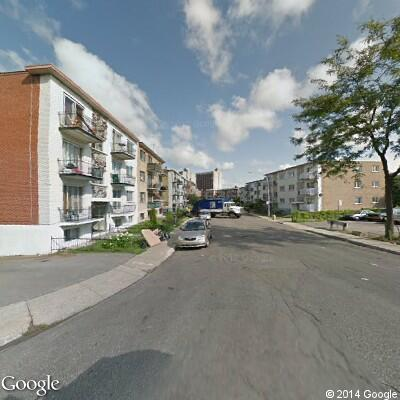
\includegraphics[width=0.21\linewidth]{montrealnord3.png}};

\onslide<2>\node (tdowntown) at (0,-1) [draw=black, thick, fill=white, scale=0.9] {Downtown};
\node (tchinatown) [right =2.7 of tdowntown] [draw=black, thick, fill=white, scale=0.9] {Chinatown};
\node (toldmont) [right =2.7 of tchinatown] [draw=black, thick, fill=white, scale=0.9] {Old Montreal};
\node (tgayvil) [below=2.7 of tdowntown] [draw=black, thick, fill=white, scale=0.9] {Gay Village};
\node (toutremont) [right=2.7 of tgayvil] [draw=black, thick, fill=white, scale=0.9] {Outremont};
\node (tplat) [right=2.7 of toutremont] [draw=black, thick, fill=white, scale=0.9] {Plateau};
\node (twest) [below=2.7 of tgayvil] [draw=black, thick, fill=white, scale=0.9] {Westmount};
\node (thoch) [right=2.7 of twest] [draw=black, thick, fill=white, scale=0.9] {Hochelaga};
\node (tnorth) [right=2.7 of thoch] [draw=black, thick, fill=white, scale=0.9] {Montreal-Nord};
%7933 7905 7882 7874 7868
\end{tikzpicture}
\end{frame}

\begin{frame}
\frametitle{Image Acquisition}
\begin{columns}[c] % The "c" option specifies centered vertical alignment while the "t" option is used for top vertical alignment

\column{.45\textwidth} % Left column and width
\begin{itemize}
\item Google Street View API
\item Use geographical coordinates of polygons defining each neighbourhood
\item 8000 100$\times$100 images per class
\item Greyscale
\end{itemize}
\column{.5\textwidth} % Right column and width
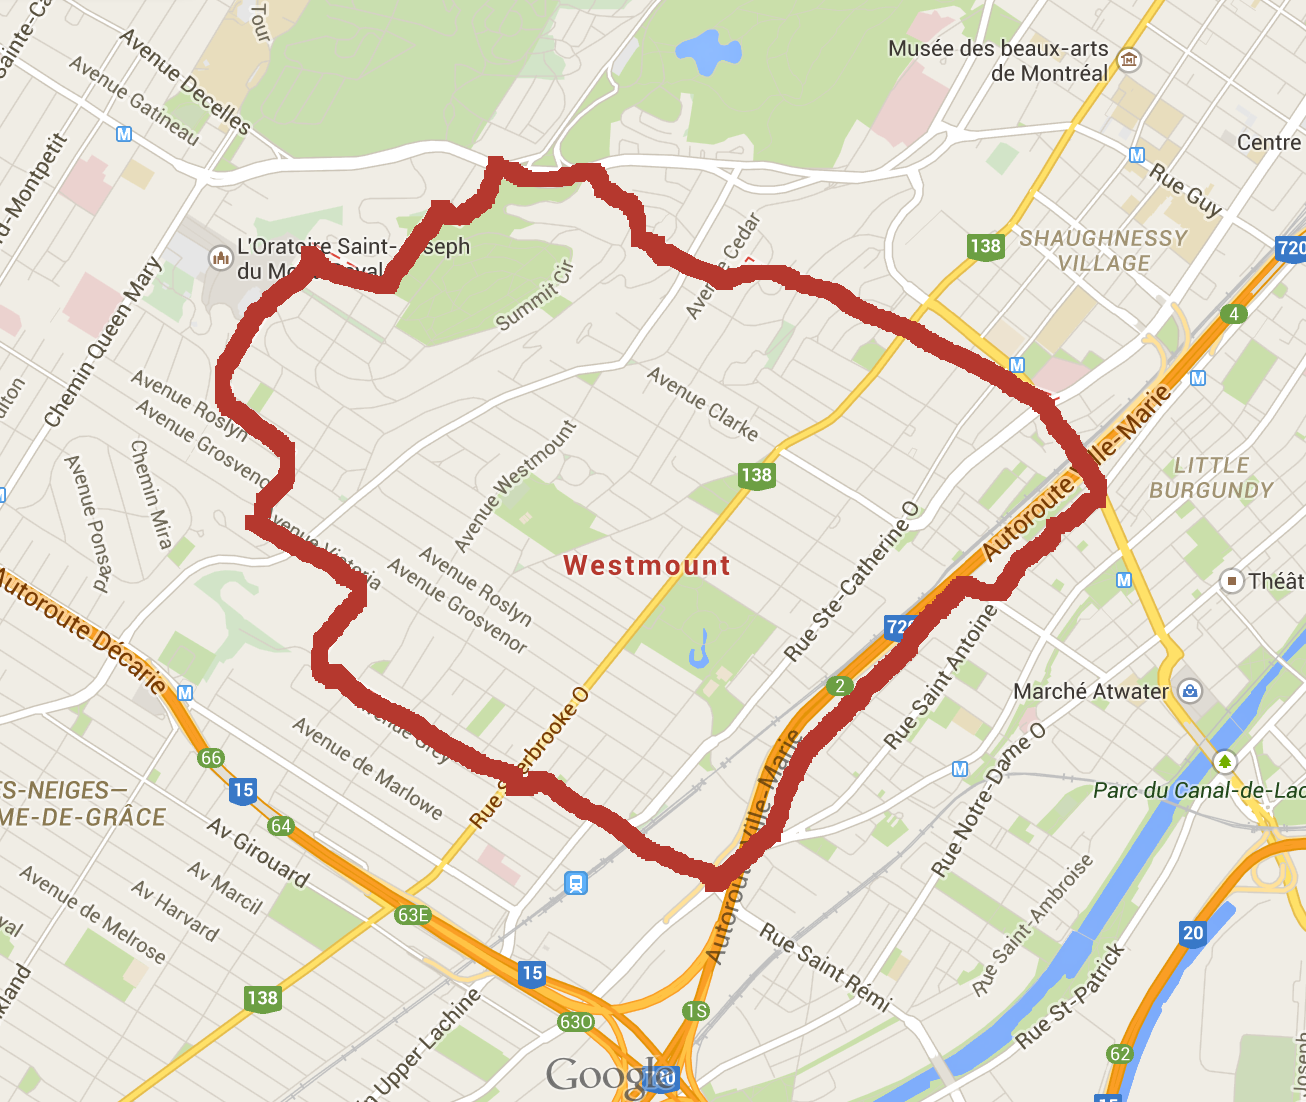
\includegraphics[width=0.9\linewidth]{polygon.png}
\end{columns}
\end{frame}

\begin{frame}
\frametitle{Machine Learning}
We compare the following techniques:
\begin{itemize}
\item Logistic regression
\item Stacked autoencoder 
\item Convolutional neural network
\end{itemize}
\end{frame}

\begin{frame}
\frametitle{Preliminary Results}

\only<1>{\begin{block}{Logistic regression}
SHITTY RESULTS
\end{block}}

\only<2>{\begin{block}{Stacked autoencoder}
\centering
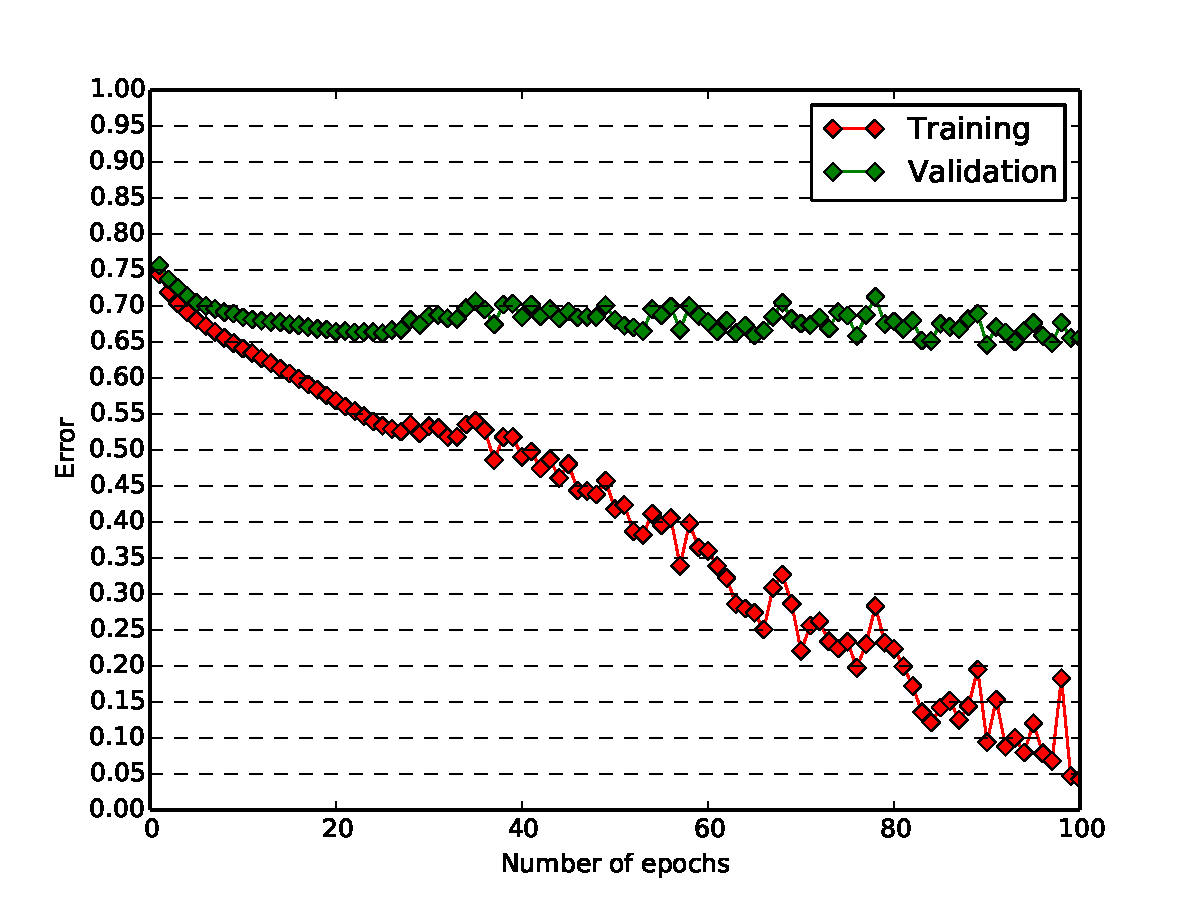
\includegraphics[width=0.75\linewidth]{best_autoencoder_learning.pdf}
\end{block}}

\only<3-4>{\begin{block}{Convolutional neural network}
\centering
\only<3>{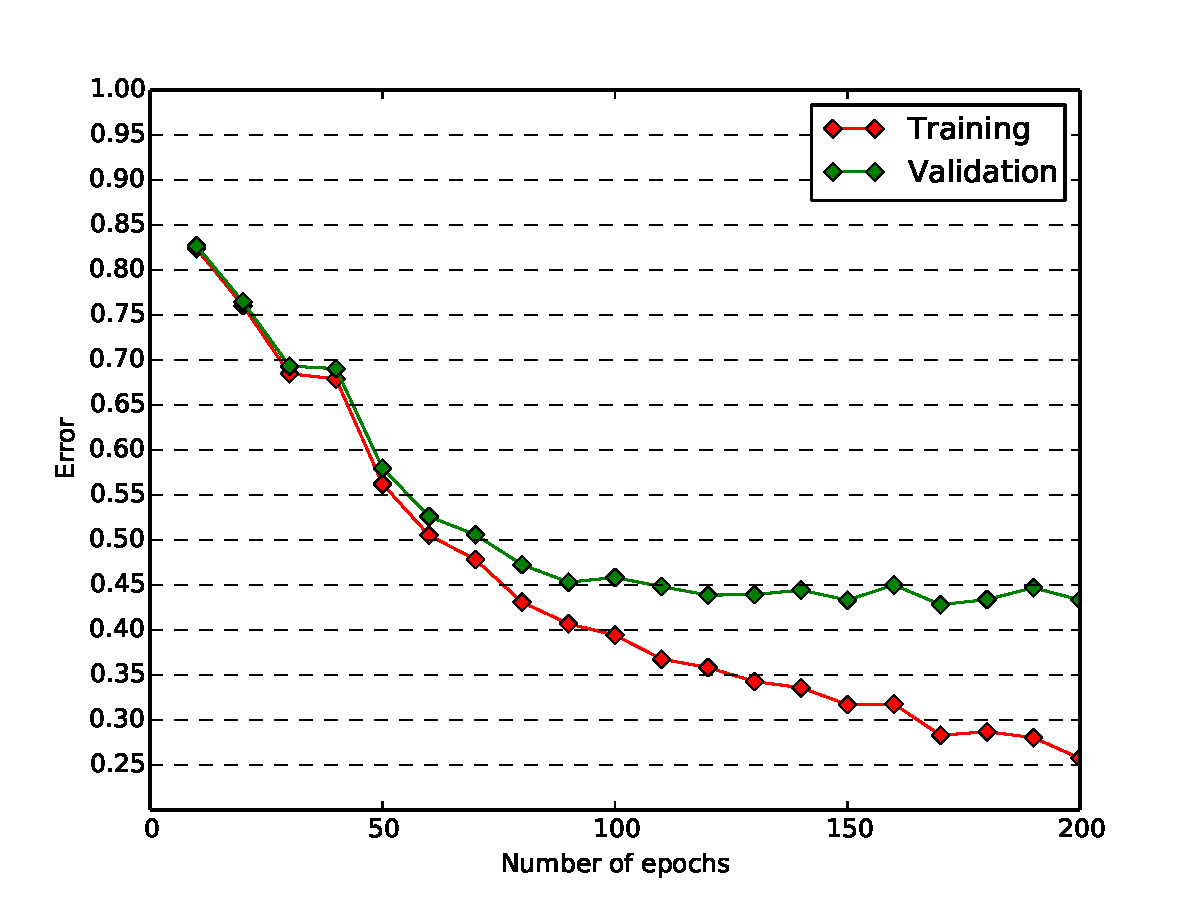
\includegraphics[width=0.75\linewidth]{best_convnet_learning.pdf}}
\only<4>{
\begin{tikzpicture}
\node (conf) at (0,0) {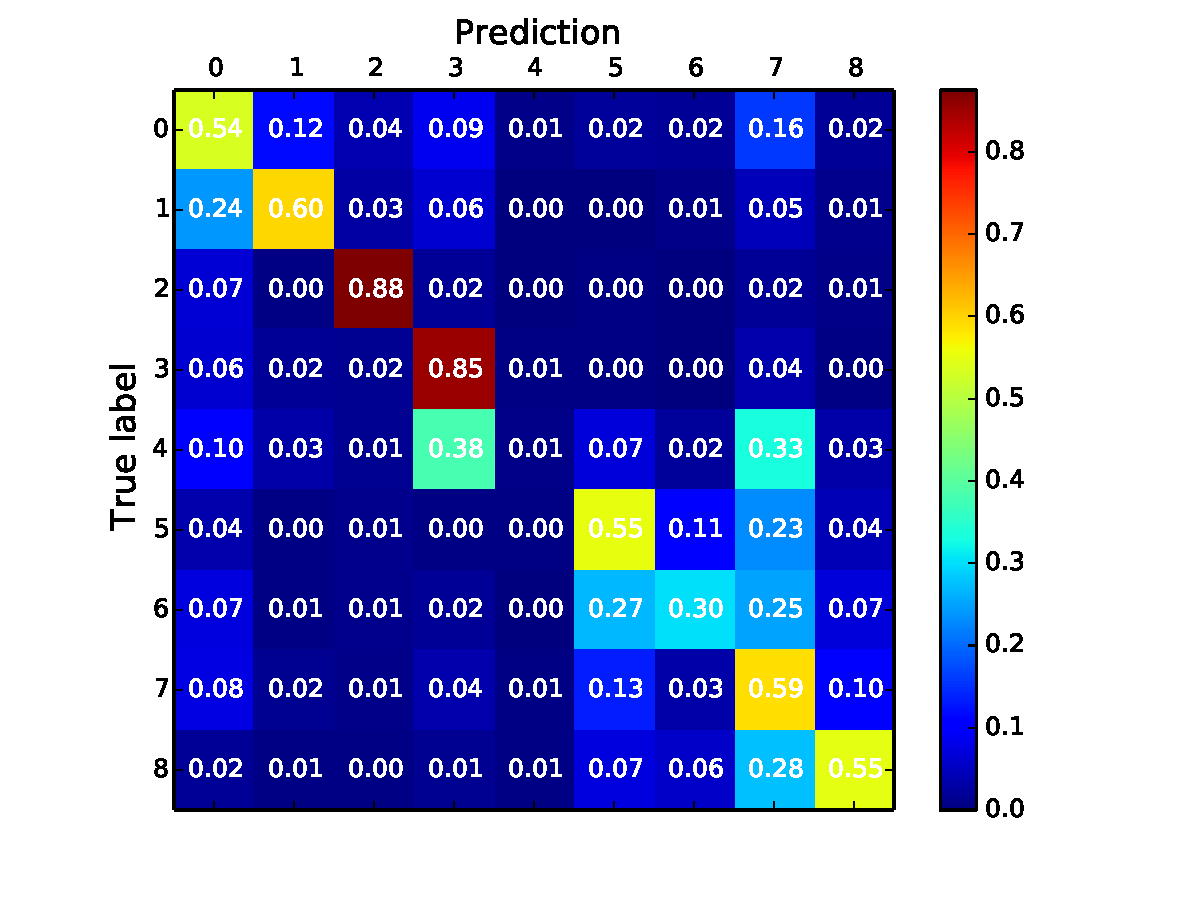
\includegraphics[width=0.6\linewidth]{convnet_confusion.pdf}};
\node (tbl) [right = 0.75 of conf, scale=0.8, draw=black, rounded corners, fill=white] {
\begin{tabular}{ l l }
Label & Borough \\ \hline
0 & Downtown \\
1 & Old Montreal \\
2 & Chinatown \\
3 & Gay Village \\
4 & Plateau \\
5 & Outremont \\
6 & Westmount \\
7 & Hochelaga \\
8 & Montreal-Nord \\
\end{tabular}};
\end{tikzpicture}
}
\end{block}}
\end{frame}

\begin{frame}
\frametitle{Outtakes}
% some weird images.
% discard images without street view
Sometimes Google Street View is Google Indoors View...
\centering
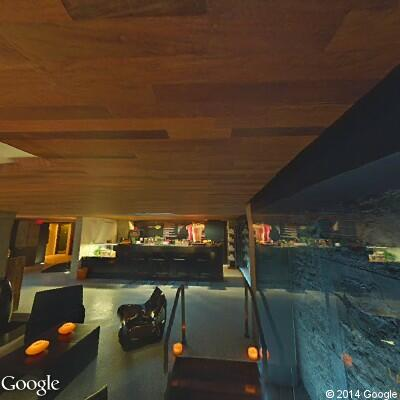
\includegraphics[width=0.6\linewidth]{indoors.png}
\end{frame}
%------------------------------------------------

%------------------------------------------------

\begin{frame}
\centering
\begin {tikzpicture}
\node (the end) at (0,0) {\Huge The End};
\draw [draw=dark green, thick, fill=dark green!40] (1, 1) circle (0.4cm);
\draw [draw=red, thick, fill=red!40] (2,2) circle (0.3cm);
\draw [draw=dark green, thick, fill=dark green!40] (3,2.5) circle (0.25cm);
\draw [draw=red, thick, fill=red!40] (4, 2.75) circle (0.2cm);
\draw [draw=dark green, thick, fill=dark green!40] (5, 2.875) circle (0.15cm);

\draw [draw=dark green, thick, fill=dark green!40] (-1,-1) circle (0.4cm);
\draw [draw=red, thick, fill=red!40] (-2,-2) circle (0.3cm);
\draw [draw=dark green, thick, fill=dark green!40] (-3, -2.5) circle (0.25cm);
\draw [draw=red, thick, fill=red!40] (-4, -2.75) circle (0.2cm);
\draw [draw=dark green, thick, fill=dark green!40] (-5, -2.875) circle (0.15cm);
\end{tikzpicture}
\end{frame}

%----------------------------------------------------------------------------------------

\end{document} 